\chapter{Modelo dinámica neuronal}\label{cap:modeloneuronal}
\graphicspath{{figs/capitulo_modelo_dinamica_neuronal/}}

\chapterquote{We shall assume. . .\\
	. . . that all cows are spherical.
}{old joke}




Una neurona de picos transforma un gran conjunto de trenes de picos de entrada de diferentes neuronas en un tren de picos de salida. Así, a nivel microscópico, los circuitos neuronales del cerebro codifican y procesan información a través de patrones de picos espaciotemporales. Se puede suponer que la dinámica de las neuronas en pico es capturada correctamente por modelos de neuronas de tipo punto de un compartimento, como el modelo de integración y disparo con fugas (LIF)81

Un gran interés en la neurociencia es comprender cómo las funciones cerebrales macroscópicas, como la cognición y la memoria, se codifican en la microescala de las neuronas y sus conectividades topológicas. n el modelo LIF, cada neurona se puede describir completamente en términos de una única variable interna, a saber, la despolarización de la membrana neural. El circuito básico de un modelo LIF consiste en un capacitor en paralelo con una resistencia impulsada por una corriente sináptica (potencial postsináptico excitatorio o inhibitorio (EPSP o IPSP), respectivamente). Cuando el voltaje a través del capacitor alcanza un umbral, el circuito se desvía y se genera un pico que se transmite a otras neuronas. En el cerebro, las redes neuronales locales comprenden un gran número de neuronas que están masivamente interconectadas. La dinámica puede describirse adecuadamente mediante un conjunto de ecuaciones diferenciales acopladas correspondientes a un modelo LIF para cada neurona. Las simulaciones directas de estas ecuaciones producen un patrón espaciotemporal complejo que cubre la trayectoria individual del estado interno de cada neurona en la red. Estos tipos de simulaciones directas son computacionalmente costosos, lo que hace que sea muy difícil analizar cómo se relaciona la conectividad subyacente con varias dinámicas.  

Los conjuntos de neuronas motoras y la organización columnar en la corteza visual y somatosensorial son ejemplos de estos conjuntos. 



\section{Medios excitables}\label{sec:mediosexcitables}



La excitabilidad se observa en una amplia gama de sistemas naturales. Una lista de ejemplos incluye láseres, reacciones químicas, canales iónicos, sistemas neuronales, tejidos cardiovasculares y dinámica del clima, por mencionar solo los campos de investigación más importantes [1], [2], [3], [4], [5] , [6], [7], [8], [9], [10], [11], [12], [13], [14], [15], [16]. Común a todos los sistemas excitables es la existencia de un estado de "reposo", un estado "excitado" (o de "disparo") y un estado "refractario" (o de "recuperación"). Si no se perturba, el sistema reside en el estado de reposo; pequeñas perturbaciones dan como resultado solo una respuesta lineal de pequeña amplitud del sistema (cf. Fig. 1a). Sin embargo, para una perturbación lo suficientemente fuerte, el sistema puede salir del estado de reposo, pasando por los estados de cocción y refractario antes de volver a descansar (Fig. 1b y c). Esta respuesta es fuertemente no lineal y está acompañada por una gran excursión de las variables del sistema a través del espacio de fase, lo que corresponde a un pico. El sistema es refractario después de un pico de este tipo, lo que significa que se necesita un cierto tiempo de recuperación antes de que otra excitación pueda provocar un segundo pico (Fig. 1d y e).


% importante galan_how_2008

La idea de que la dinámica neuronal codifica y almacena representaciones de estímulos en forma de atractores de la dinámica de redes ha sido alimentada por los hallazgos de varios estudios experimentales en diferentes sistemas [7,30–33]. Además, se ha propuesto recientemente que los estados ascendentes de red altamente consistentes y evocados espontáneamente observados en cortes corticales representan atractores de circuitos [1,4]. Aquí, hemos demostrado que los componentes principales de la actividad espontánea pueden interpretarse como atractores de la actividad de fondo estocástica de la red. En particular, los valores propios de la matriz de covarianza representan aproximadamente la fracción de tiempo que la red pasa en la cuenca de atracción (tiempo de permanencia) del vector propio asociado o componente principal. Además, los cambios en el componente principal de la actividad espontánea durante los experimentos de comportamiento se pueden utilizar para cuantificar los cambios en la conectividad de la red y, por lo tanto, descubrir las huellas de la memoria hebbiana, como se mostró recientemente en el cerebro de un insecto in vivo [7]




Algunos de estos ejemplos se pueden representar como sistemas "excitables". El concepto de medio excitable fue introducido por Wiener y Rosenbluth (1946) para explicar las arritmias cardíacas causadas por ondas espirales. Inventaron las notaciones de los estados refractario, excitable y excitado. Las características definitorias de los sistemas excitables son: (i) comenzando en un equilibrio estable (estado de reposo), un estímulo por encima de cierto umbral genera (ii) un estallido de actividad (estado excitado) seguido de (iii) un período refractario (estado de recuperación) .

los tejidos neuronales y musculares hechos de células animales pueden generar y propagar señales electrofisiológicas. Estas células pueden excitarse en respuesta a estímulos externos provenientes de células cercanas, y pueden generar un potencial de acción a través de sus membranas celulares que se transmitirá como estímulo a otras células cercanas. Una vez excitada, la célula pasa por un periodo refractario durante el cual no responde a ningún otro estímulo. Esto provoca la direccionalidad de la propagación de la señal y la formación de \textquote{ondas viajeras} en los tejidos. El medio por el cual es posible este tipo de ondas es un medio excitable. 

\section{refractario}


En general, las conductancias reguladas por voltaje y calcio suelen conducir a estados refractarios, que pueden ser cortos después de picos individuales o más largos después de períodos de actividad más intensos.

En muchos sentidos, este medio químico se comporta como el sistema sexual humano. respuesta. La excitación sexual y la recuperación dependen de las propiedades del tejido nervioso que, como la sopa Zhabotinslcy, pertenece a una clase general de sistemas llamados medios excitables. Una neurona tiene tres estados: inactivo, excitado y refractario. Normalmente una neurona está quiescente. con estimulación inadecuada, muestra poca respuesta y vuelve al reposo. Pero un estímulo suficientemente provocador excitará a la neurona y la hará disparar. Luego se vuelve refractario (incapaz de ser excitado por un tiempo) y finalmente vuelve a la inactividad. Los paralelos con las ondas químicas se extienden a los potenciales de acción, las ondas eléctricas que se propagan a lo largo de los axones nerviosos. Ellos también viajan sin atenuación, y cuando algunos de ellos chocan, se aniquilan entre sí. De hecho, todas estas afirmaciones son igualmente ciertas para las ondas eléctricas en otro medio excitable: el corazón. Esa es la belleza de esta abstracción: las propiedades cualitativas de un medio excitable valen para todos. Todos se pueden estudiar de un solo golpe. El parecido de familia entre la sopa de Zhabotinsky, el tejido nervioso y el músculo cardíaco persiste hasta la estructura de las ecuaciones matemáticas que gobiernan su dinámica no lineal. La analogía es profunda.




La excitabilidad se observa en una amplia gama de sistemas naturales. Una lista de ejemplos incluye láseres, reacciones químicas, canales iónicos, sistemas neuronales, tejidos cardiovasculares y dinámicas climáticas, por mencionar sólo los campos de investigación más importante. Todos los sistemas excitables tienen en común la existencia de un estado de "reposo", un estado de "excitación" (o "disparo") y un estado "refractario" (o de "recuperación"). Si no se perturba, el sistema permanece en estado de reposo; pequeñas perturbaciones sólo dan lugar a una respuesta lineal del sistema de pequeña amplitud (véase la Fig. 1a). Sin embargo, para una perturbación suficientemente fuerte, el sistema puede abandonar el estado de reposo, pasando por los estados de disparo y refractario antes de volver de nuevo al estado de reposo (Fig. 1b y c). Esta respuesta es fuertemente no lineal y va acompañada de una gran excursión de las variables del sistema a través del espacio de fases, lo que corresponde a un pico. El sistema es refractario después de un pico de este tipo, lo que significa que necesita un cierto tiempo de recuperación antes de que otra excitación pueda evocar un segundo pico (Fig. 1d y e).



La respuesta de un elemento excitable (por ejemplo, una neurona, una célula cardíaca o ciertos dispositivos artificiales) a un estímulo finito comienza con un estallido no lineal de actividad: la etapa excitada. Le sigue una disminución de la actividad por debajo de su nivel de referencia, durante la cual el elemento es insensible a los estímulos, de ahí el nombre de etapa refractaria para esta fase. Luego, el elemento vuelve a su estado de referencia estable y permanece en este estado de reposo hasta que experimenta otro estímulo. El hecho notable acerca de las unidades excitables reales es que la duración, forma y amplitud de la secuencia dinámica estimulada es casi insensible al estímulo, siempre que sea lo suficientemente fuerte. Esta característica invariable de todo o nada conduce a la descripción de la conducta excitable mediante una dinámica determinista, de tiempo discreto y simbólica.


Su comportamiento se caracteriza por la existencia de un umbral de activación tal que pequeñas fluctuaciones sobre el estado de reposo del sistema decaen rápidamente sin tener ningún efecto sobre el sistema. Sólo un estímulo fuerte, es decir, que supere el umbral, es capaz de hacer que el sistema pase a otro estado distinto del estado de reposo, denominado estado “activado” o “excitado”. na vez que un elemento en este sistema alcanza su estado excitado, permanece allí solo por una duración finita antes de regresar lentamente a su estado de reposo en equilibrio dentro de un intervalo de tiempo conocido como el "período refractario". Durante este tiempo, el elemento no puede ser reexcitado ni siquiera con un estímulo superior al umbral. La consecuencia un tanto inesperada del período refractario es que cuando dos ondas en un medio excitable chocan de frente, se aniquilan entre sí.


Otra consecuencia es que una onda con un frente roto (es decir, una singularidad en el extremo roto de la onda que tiene en su vecindad puntos pertenecientes a cada fase del ciclo, desde los estados de reposo hasta los estados activados y refractarios) se enrollará para formar el forma de gancho de una onda espiral que se mueve continuamente hacia afuera desde la singularidad central (la fuente de la onda). Otra manifestación de este fenómeno se observa en las colonias del moho mucilaginoso celular, Dictyostelium, donde la falta de nutrientes puede desencadenar la secreción de monofosfato de adenosina cíclico (cAMP). Esto da como resultado ondas espirales de cAMP que se propagan a través de la colonia, lo que indica a las diferentes células que comiencen a agregarse para formar un organismo multicelular.

Entonces, el estado excitado es metaestable, en el sentido de que el sistema regresa espontáneamente al estado de reposo. El estado de reposo, por otro lado, es un equilibrio estable del cual el sistema puede ser desplazado solo por una perturbación lo suficientemente grande. Cualquier medio excitable comparte estas cualidades: tiene un estado de reposo estable y un estado excitado metaestable; la transición de la primera a la segunda solo puede tener lugar si hay una perturbación externa cuya magnitud está por encima de un cierto umbral. Otra propiedad de un medio excitable es la existencia de un período refractario. Una vez que el medio ha sido excitado, tarda un tiempo en recuperarse, tiempo durante el cual el sistema no puede ser reexcitado por otro estímulo superior al umbral.



Estas dos propiedades clave de tener (i) un estado excitado metaestable que se puede alcanzar solo cuando se aplica una estimulación superior a un valor umbral, y (ii) un período refractario inmediatamente después de la excitación durante el cual la reexcitación no es posible, incluso con estimulación mucho mayor que el valor umbral, dan lugar a una serie de características interesantes. Uno de ellos es que viajan ondas de excitación. Una de ellas es que las ondas viajeras de excitación en dicho medio no pueden atravesarse entre sí. Cuando dos de esas olas se encuentran, se aniquilan mutuamente. La razón es que detrás de los frentes de onda se encuentran regiones que se encuentran en sus períodos refractarios y no pueden ser excitadas. Por lo tanto, los frentes de onda de excitación no pueden cruzarse entre sí \cite{sinha_patterns_2019}. 




Los medios excitables espacialmente extendidos son una subclase dentro del marco más general de los sistemas de reacción-difusión. Como sugiere el nombre, los modelos de reacción-difusión proporcionan una descripción natural de la dinámica de un sistema químico: los reactivos reaccionan entre sí y los reactivos y los productos se transportan a través de la difusión \cite{sinha_patterns_2019}. Con el tiempo, estos modelos se han utilizado para analizar una amplia clase de sistemas espacialmente extendidos en química, física, biología y ecología [Cross y Greenside 2009; Cruz y Hohenberg 1993; Murray 2002]. Bajo granularidad gruesa, estos sistemas se modelan usando ecuaciones diferenciales parciales (PDEs) que tienen la forma:


También vale la pena discutir la dinámica de los medios excitables porque juegan un papel central en muchas cuestiones fascinantes y oportunas relacionadas con la biología, la fisiología y la medicina (también en química e ingeniería química, como la propagación de ondas químicas en la superficie de un metal). Catalizador). Por lo tanto, incluso los organismos unicelulares, como un paramecio, han evolucionado para crear ondas eléctricas excitables a lo largo de su membrana y usan estas ondas para controlar la rotación mecánica de sus cilios y, por lo tanto, sus movimientos de natación. Una onda eléctrica excitable juega un papel importante en la fusión de un espermatozoide con un óvulo; la ola desencadena un rápido cambio en la membrana del óvulo que impide la entrada de un segundo espermatozoide, lo que entorpecería el desarrollo del organismo. Los organismos multicelulares han desarrollado sistemas nerviosos en los que la información se transmite de una neurona a otra (o de las neuronas a los músculos) en forma de pulsos breves a través de conexiones excitables unidimensionales especializadas llamadas axones. En el caso de un animal grande como una ballena azul, estos pulsos podrían propagarse decenas de metros sin disminuir la amplitud o la velocidad, un logro evolutivo notable.
Las neuronas y el músculo cardíaco son sistemas excitables clásicos con la propiedad de que una perturbación de pequeña amplitud (correspondiente, por ejemplo, a la inyección de una pequeña cantidad de corriente a través de un electrodo de metal) decae mientras que una perturbación que hace que el voltaje a través de la membrana de una célula exceda un cierto El umbral provoca una gran respuesta amplificada rápida, lo que conduce a un pulso que puede propagarse largas distancias sin decaer o cambiar de forma \cite{cross_pattern_2009}. 

% Emergence of Asynchronous Local Clocks in Excitable Media
Los medios excitables, como el miocardio o el cerebro, consisten en conjuntos de elementos excitables acoplados, en los que la excitación local de un solo elemento puede propagarse a sus vecinos en forma de autoonda no lineal. Dado que cada elemento tiene que pasar por un período refractario inmediatamente después de la excitación, la frecuencia de las ondas automáticas es autolimitante. Las oscilaciones autoorganizadas son omnipresentes en sistemas complejos que consisten en elementos excitables distribuidos con interacciones no lineales. Un ejemplo bien conocido son las reacciones de Belousov-Zhabo-tinsky [1, 2], en las que los cambios de color cíclicos y otros patrones espaciotemporales surgen de procesos de reacción química simples. Un fenómeno típico en este tipo de sistemas es la denominada autoonda, una propagación de excitación similar a una onda entre los elementos individuales que no obedece al principio de superposición lineal. En este contexto, la "excitación" de un elemento se puede definir como un estado particular del elemento, de un conjunto discreto de estados posibles.


Estudios experimentales en la década de 1950 de axones gigantes de calamar, que tienen aproximadamente 1 mm de diámetro2 (ver Fig. 1.1), llevaron a la primera comprensión cuantitativa de cómo las neuronas se transmiten señales entre sí. La descripción teórica resultante conocida como ecuaciones de Hodgkin-Huxley continúa brindando la forma más utilizada para modelar neuronas y otros tejidos biológicos excitables como el tejido cardíaco.





Los medios excitables espacialmente extendidos son una subclase dentro del marco más general de los sistemas de reacción-difusión. Como sugiere el nombre, los modelos de reacción-difusión proporcionan una descripción natural de la dinámica de un sistema químico: los reactivos reaccionan entre sí y los reactivos y los productos se transportan a través de la difusión \cite{sinha_patterns_2019}. Con el tiempo, estos modelos se han utilizado para analizar una amplia clase de sistemas espacialmente extendidos en química, física, biología y ecología [Cross y Greenside 2009; Cruz y Hohenberg 1993; Murray 2002]. Bajo granularidad gruesa, estos sistemas se modelan usando ecuaciones diferenciales parciales (PDEs) que tienen la forma:

\begin{equation}\label{eq:74}
	\frac{\partial \mathbf{q}(\mathbf{x},t)}{\partial{t}} = \bm{D} \nabla^{2} \mathbf{q}(\mathbf{x},t)+\mathbf{R}(\mathbf{q})
\end{equation}


donde cada componente de $\mathbf{q}(\mathbf{x},t)$ representa una de las diversas variables que describen el estado de un sistema (por ejemplo, la concentración de una especie química en caso de reacciones químicas),  $\bm{D}$  es la matriz de difusión y $\mathbf{R}(\mathbf{q})$ representa la diferentes términos de reacción (no lineales). Por lo tanto, el término del lado derecho de la \cref{eq:74} representa el transporte de los diferentes componentes, mientras que el segundo término contiene detalles de todos los procesos dinámicos locales que operan en cada uno de los componentes, incluida la producción, la descomposición, etc \cite{sinha_patterns_2019}.



Además de los patrones de Turing, los sistemas de reacción-difusión pueden exhibir una amplia gama de otros comportamientos dinámicos espaciotemporales, como ondas viajeras, solitones disipativos, caos espaciotemporal, etc. Si bien algunos de estos pueden explicarse mediante un tratamiento analítico, se debe recurrir a métodos numéricos. simulaciones para estudiar el resto. el primer paso es la discretización del laplaciano u operador de difusión para un sistema finito que convierte el espacio continuo en una red discreta. Por lo tanto, este proceso convierte un sistema de EDP en un gran número de ecuaciones diferenciales ordinarias (EDO) acopladas. La difusión ahora está representada por el acoplamiento de variables adecuadas en un punto de red dado con las de sus vecinos más cercanos \cite{sinha_patterns_2019}.






Tradicionalmente, se supone que el espacio continuo (y, por tanto, el sistema de EDO) representa la realidad, mientras que la red (en consecuencia, el sistema de EDPs acopladas) se considera una aproximación.Sin embargo, con la tecnología moderna es posible investigar sistemas donde la red espacialmente discreta es la descripción más precisa y la PDE correspondiente es una aproximación \cite{sinha_patterns_2019}.

Como se mencionó en el Prefacio, los modelos de medios excitables forman una clase especial dentro del marco proporcionado por el sistema de reacción-difusión. Un rasgo característico que distingue a la mayoría de los sistemas excitables es que surgen patrones a través de la interacción entre ondas de actividad transitoria que se propaga a través del medio. Uno de los primeros sistemas donde se analizó en detalle la existencia de ondas de excitación en propagación es el axón gigante del calamar. La transmisión de impulsos nerviosos en esta célula fue estudiada mediante técnicas de electrofisiología por Hodgkin y Huxley. También proporcionaron una base para describir dicha actividad en términos de modelos matemáticos que forman la base de todo el trabajo teórico posterior sobre sistemas excitables.



En muchas aplicaciones, la descripción matemática de los procesos dinámicos en un medio excitable se representa en forma de un sistema de reacción-difusión de $N$ componentes,


\begin{equation}\label{eq:54}
	\frac{\partial E_i}{\partial t} = \nabla \cdot \left(D_i\nabla\vec{E}\right) + F_i \left(\vec{E}\right),
\end{equation}

Aquí el vector $\vec{E}$ determina el estado del sistema, y los $F_i$ son funciones no lineales de $\vec{E}$. Los $D_i$ son coeficientes de difusión. Los ejemplos más famosos incluyen el modelo de Hodgkin-Huxley para el axón gigante del calamar, el modelo de Noble para las fibras de Purkinje, el modelo de Fenton-Karma para el tejido cardíaco, el modelo de Oregonator para la reacción química de  Belousov-Zhabotinsky ( BZ) , el modelo de Martiel-Goldbeter para la señalización de AMPc en células de Dictyostelium, etc \cite{zykov_wave_2018}.

% Wave Propagation in Inhomogeneous Excitable Media
Un medio excitable es un sistema dinámico no lineal distribuido continuamente en el espacio, cada segmento elemental del cual es susceptible de ser activado; es decir, posee la propiedad de excitabilidad. Los segmentos vecinos de un medio excitable interactúan entre sí mediante procesos de transporte local similares a la difusión. En tal medio, una excitación activada dentro de un área restringida puede propagarse de un segmento a otro por medio de acoplamiento local. Por lo tanto, un medio excitable admite la propagación de ondas de excitación solitarias no amortiguadas. Dicha onda consiste en una transición rápida de un estado de reposo estable a un estado excitado (frente de onda) seguido de una meseta y finalmente por una transición de recuperación (onda de regreso) hacia el estado de reposo.


Un ejemplo típico de excitabilidad es la generación de un pico de potencial transmembrana (potencial de acción) por una célula cardíaca, inducida por una breve perturbación eléctrica despolarizante de un estado de reposo. Por lo general, la forma del potencial de acción generado no depende de la fuerza de la perturbación, siempre que la perturbación supere algún umbral (principio de todo o nada). Después de la generación de esta fuerte respuesta, el sistema vuelve a su estado de reposo inicial. Se puede generar una excitación posterior después de que haya pasado un período de tiempo adecuado, denominado período refractario. Debido a esta característica, un medio es capaz de soportar no solo ondas de excitación solitarias sino también trenes de ondas. La descripción de las reglas dinámicas que gobiernan las neuronas a nivel microscópico [4] y la primera demostración matemática de una transición de fase de segundo orden en un sistema de muchos cuerpos [5] fueron casi contemporáneas. Sin embargo, estos desarrollos estuvieron separados por una gran brecha temporal de las primeras propuestas de criticidad en la dinámica cerebral [2, 6]. Siendo una propuesta relativamente reciente, las consecuencias de tal hipótesis aún están lejos de ser claras. En el presente ensayo, primero discutimos la evidencia empírica reciente que favorece esta hipótesis, centrándonos en la presencia de una transición de fase de segundo orden en la dinámica cerebral a gran escala [7], y luego exploramos algunas posibles consecuencias. 


% Stochastic cellular automata modeling of excitable systems
Un comportamiento genérico de los medios excitables es producir ondas químicas de varias geometrías, viajando en el sistema [133,134]. Las ondas anulares y espirales son un patrón típico de excitaciones. Muchos sistemas químicos exhiben un comportamiento excitable. El modelo de Selkov [135] y la reacción de Belousov-Zhabotinsky son ejemplos. Las ondas químicas juegan un papel importante en muchos procesos biológicos (sistema nervioso, músculos) ya que pueden mediar en el transporte de información de un lugar a otro. El modelo de Greenberg-Hasting es un ejemplo de modelo de autómata celular de un medio excitable. Esta regla, y su generalización, han sido extensamente estudiadas [136,137].

Uno de los ejemplos más extraños del mundo real de un medio excitable es la transmisión de ondas de \gls{AMP} cíclico en la fase de agregación de amebas" del moho mucilaginoso Dictyostelium discoideum (ver \Cref{fig:hongo}). Más tarde, esta criatura se convierte en una babosa multicelular.  Comenzando con el trabajo seminal de Wiener y Rosenblueth 1946, e impulsado por el descubrimiento de la reacción química oscilante de Belousov Zhabotinski a finales de los años sesenta, se ha desarrollado un cuerpo considerable de conocimiento sobre el tema de los medios excitables. 

\begin{figure}[ht]
	\centering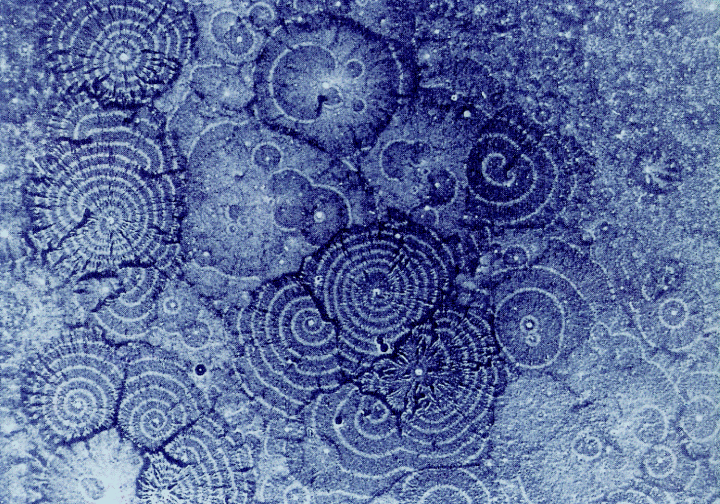
\includegraphics[width=\imsize]{hongo.png}
	\caption[Diagrama que muestra el patrón creado por el \gls{AC} regla 30, con celdas coloreadas según el estado anterior de su vecindad. ]{Patrón de reacción de Belousov-Zhabotinskii (BZ) en la agregación de Dictyostelium amebae. Los patrones de ondas espirales y ondas concéntricas que caracterizan la reacción BZ pueden verse claramente. Las bandas claras y oscuras surgen de las diferentes propiedades ópticas entre las amebas en movimiento y las estacionarias. Las células se ven brillantes cuando se mueven y oscuras cuando están estacionarias. El área es de \qtyproduct{6x 8}{\centi\metre}. La fotografía es cortesía del Dr. Peter C. Newell (Departamento de Bioquímica, Universidad de Oxford, Oxford, Reino Unido).} 	\label{fig:hongo}
\end{figure}


Si un medio excitable es bidimensional (es decir, una lámina de medio o una capa muy delgada), se pueden observar varias geometrías de ondas fundamentalmente diferentes.  En uno, las ondas se originan en una fuente puntual (por ejemplo, el lugar donde un rayo inició un incendio forestal) y se propagan en círculos concéntricos.  Otra geometría de ondas involucra la propagación de ondas espirales de actividad (ver Figura 2.12). Aquí la onda se mueve en un circuito aunque no haya un agujero en el medio. En cambio, la onda se forma en una espiral y el "agujero" es funcional creado de momento a momento por áreas de medio refractario. Las espirales pueden ser estables, o pueden serpentear en geometrías complejas, o incluso pueden dividirse en múltiples espirales (ver Figura 2.26).


Los medios excitables denotan una clase de sistemas que comparten un conjunto de características que hacen que su comportamiento dinámico sea cualitativamente similar. Estas características incluyen (i) la existencia de dos estados dinámicos característicos, que comprenden un estado de reposo estable y un estado excitado metaestable, (ii) un valor umbral asociado con una de las variables dinámicas que caracterizan el sistema, al exceder el cual, el sistema cambia de el estado de reposo al estado excitado, y (iii) un período de recuperación después de una excitación, durante el cual la respuesta del sistema a un estímulo superior al umbral disminuye, si no desaparece por completo
Los sistemas naturales que exhiben tales características incluyen, en biología, células tales como neuronas, miocitos cardíacos y células beta pancreáticas, todas las cuales son vitales para la función de un organismo vivo complejo [2]. Otros ejemplos de fenómenos dinámicos asociados con medios excitables incluyen ondas de AMPc observadas durante la agregación de moho mucilaginoso [3], ondas de calcio intracelular observadas en ovocitos de Xenopus [4], contracciones musculares durante el parto en tejido uterino [5], ondas de calcio intercelular en cortes de cerebro [6, 7], ondas químicas observadas en la reacción de Belusov-Zhabotinsky [8] y patrones de concentración en la reacción de oxidación de CO en la superficie de Pt(110) [9] La excitación en tales sistemas se observa como un potencial de acción característico, donde una variable asociada con el sistema (por ejemplo, el potencial de membrana, en el caso de las células biológicas) aumenta rápidamente desde su valor de reposo hasta el valor máximo correspondiente al estado excitado, seguido de un proceso más lento durante el cual vuelve gradualmente al estado de reposo.

\subsection{Modelo de Fitzhugh-Nagumo}\label{modelo_Fitzhugh-Nagumo}
Uno de los sistemas modelo más simples capaz de exhibir todas estas características es el sistema genérico de Fitzhugh-Nagumo de dos ecuaciones diferenciales acopladas.

\begin{align}\label{eq:75}
	\frac{\partial e}{\partial t}&=e(1-e)(e-b)-g,\\
	\frac{\partial g}{\partial t} &= \epsilon (ke-g).
\end{align}

Al tener solo dos variables, dicho sistema es obviamente incapaz de exhibir caos. Sin embargo, cuando varios de estos elementos excitables se acoplan para simular un medio extendido espacialmente, por ejemplo, una pieza de tejido biológico compuesta por una gran cantidad de células, el sistema dinámico de alta dimensión resultante puede mostrar un comportamiento caótico bajo ciertas condiciones 1 . La génesis de este caos espaciotemporal radica en la propiedad distinta de las ondas que interactúan en medios excitables, que se aniquilan mutuamente al chocar. Esto es consecuencia de que la región inmediatamente detrás del frente de onda de excitación consiste exclusivamente en células que están todas en la fase de recuperación. Por lo tanto, estas células en la onda de retorno no pueden ser estimuladas por otro frente de onda de excitación cuando dos de esas ondas se encuentran e intentan cruzarse entre sí 2 . Como resultado, la colisión de dos frentes de excitación conduce a la aniquilación mutua.


La interacción entre tales ondas da como resultado la creación de patrones espaciales, denominados de diversas formas excitaciones reentrantes (en 1D), vórtices u ondas espirales (en 2D) y ondas de desplazamiento (en 3D). Estos patrones se forman cuando un frente de onda de excitación se rompe cuando la onda se propaga a través del tejido parcialmente recuperado o se encuentra con un obstáculo inexcitable. Los extremos libres del frente de onda roto se enroscan gradualmente para formar ondas en espiral. Una vez formadas, estas ondas se convierten en fuentes autosuficientes de excitación de alta frecuencia en el medio y, por lo general, solo pueden detenerse mediante una intervención externa. En general, las ondas espirales se asocian con patrones periódicos o cuasiperiódicos de actividad temporal. Por lo tanto, la existencia de propiedades no lineales de propagación de ondas en varios medios excitables puede dar lugar a ritmos espaciotemporales no caóticos complejos \cite{tesis_Sridhar}.












\section{Modelo neuronal}\label{sec:modelo_dinamica_neuronal}

La dinámica cerebral se puede describir mediante muchos modelos matemáticos, tanto discretos (como los autómatas celulares, las redes booleanas, las redes booleanas probabilísticas) como continuos [como las redes neuronales celulares (CNN)50, las ecuaciones diferenciales ordinarias (EDO) o las ecuaciones diferenciales parciales (PDE)51,52]. Optamos por no usar PDE en múltiples dimensiones porque involucran dinámicas locales, que no son adecuadas para modelar las redes de conectomas descritas anteriormente. El uso de conjuntos de PDE unidimensionales también presenta dificultades. Si bien dichos sistemas describen de manera eficiente la transmisión de señales en una línea, no brindan información específica sobre cómo explicar lo que sucede en la intersección de varias líneas, que ocurren como puntos singulares. La introducción de los sistemas de Redes Neuronales Celulares (CNN), al hacer que el tiempo sea continuo pero discretizando el espacio, supera este problema, reduciendo los enlaces de red a las líneas de transmisión53–56. Dicho modelado permite no solo modelar el funcionamiento de las áreas cerebrales de interés, que respaldan varias funciones cognitivas, sino también proporcionar información sobre la capacidad de transmitir información a través de líneas de transmisión. Pero, como en este trabajo nos interesa cómo surge el proceso de generación de circuitos cognitivos para estudiar las áreas cerebrales involucradas que dan lugar a funciones cognitivas específicas, la mejor opción parecía ser adoptar una conceptualización extremadamente simple como los modelos de Redes Booleanas, que podría formar la línea de base para estudios posteriores y más complejos. Además, al usar BN versus autómatas celulares, se pueden considerar influencias en la dinámica cognitiva que no están determinadas por los vecinos inmediatos. Es obvio que pensar en el estado de regiones individuales con solo 2 valores en lugar de un estado continuo como en las CNN, o considerar el sistema determinista en sus interacciones en lugar de probabilístico, limita severamente la posible dinámica. A pesar de ello, los comportamientos que exhibe el sistema, como veremos más adelante, mantienen su complejidad, propia de sistemas computacionales que, más allá de la simpleza del modelo, exhiben comportamientos complejos o caóticos y capacidades computacionales universales 57. Así, el modelo de redes booleanas nos pareció el más adecuado para analizar el comportamiento dinámico de redes de este tipo sin perder complejidad y sin introducir elementos arbitrarios adicionales en el modelado. Hay casi 6 modelos diferentes de redes booleanas, que pueden explotarse adecuadamente para lograr diferentes dinámicas, dentro del contexto de las redes cerebrales.

% https://journals.plos.org/ploscompbiol/article?id=10.1371/journal.pcbi.1007442
Conectar la dinámica de una sola neurona con el comportamiento de la población ha sido el foco central de la investigación dentro de la comunidad de neurociencia teórica durante las últimas cuatro décadas. Los modelos de campo neuronal [ 12 - 15 ] han sido cruciales para comprender cómo la dinámica de activación macroscópica en poblaciones de neuronas emerge del estado microscópico de neuronas individuales. Dichos modelos han encontrado diversas aplicaciones, incluida la memoria de trabajo (ver [ 16 ] para una revisión), la epilepsia (p. ej., [ 17 – 20 ]) y las alucinaciones (p. ej., [ 21 – 23 ]), y se han relacionado con éxito con datos de neuroimagen como Electroencepelografía (EEG; [ 24 – 26]), magnetoencefalografía (MEG; [ 24 ]), electromiografía (EMG; [ 27 ]) y resonancia magnética funcional (fMRI; [ 25 ]), que miden señales promedio de millones de neuronas. Sin embargo, el uso de modelos de campo neuronal para modelar datos de picos de HDMEA directamente sigue siendo un problema estadístico abierto: las grabaciones de HDMEA brindan detalles suficientes para permitir el modelado de neuronas individuales, pero la gran cantidad de neuronas presentes impide la adopción de enfoques estándar para la asimilación de datos no lineales. como la inferencia libre de probabilidad.


